\chapter{Methodology}
\label{chap:3}

\section{Overview} 

Dark matter, an invisible material that comprises about 27 percent of the universe, has long been a focus of astrophysics research. It would be one of the important constituents of the universe, yet hitherto has escaped conventional detection. Dark matter is fundamental to explaining how galaxies form and the gravitational forces at work in the cosmos. The methods of study of the dark matter are based on complex analysis using supercomputers, data obtained from astronomical observations and advanced mathematical models. They are frequently based on Machine Learning (ML) algorithms aimed at helping to interpret complicated data and perform predictions of the behavior/properties of dark matter.



\section{Apparatus and Procedure for Computer Data Collection and Simulation}

For dark matter studies, data are usually obtained with sophisticated observatories and telescopes which combine multiple observations including galaxy clusters and gravitational lenses. Computer simulations are then employed to follow dark matter’s potential impact on these cosmic features. Such simulations provide a way to simulate under controlled conditions and powerfully test hypotheses about the nature of dark matter, in particular predicting how it interacts with visible matter and gravitational fields.

\section{Data Pre-processing}

Observational data obtained from different astronomical facilities may be noisy, not complete or in formats difficult to analyze. This data needs to be cleaned and processed before it is ready for analysis. Basics like cleaning noises, filling NAs, normalizing data are the most important step to avoid any distorted learning from ML models.
\section{Multivariate Analysis}
\begin{figure}[H]
    \centering
    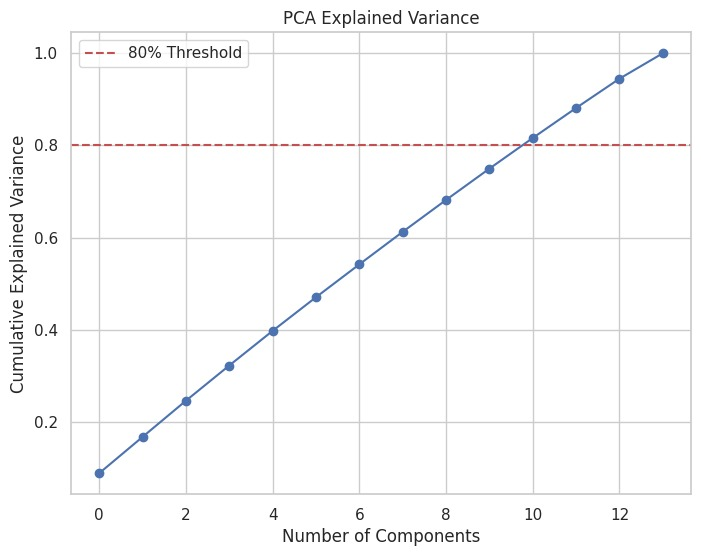
\includegraphics[width=1\linewidth]{Chap3/pca_explained_variance.jpeg}
    \caption{PCA Explained Variance}
    \label{fig:placeholder}
\end{figure}

This figure gives the Scree Plot, i.e. a cumulative variance plot of PCs from a PCA over a dataset.

\begin{itemize}
    \item The horizontal x-axis is the number of components, and the vertical y-axis is the cumulative explained variance.

    \item The figure reveals a continuous growth of the variance for higher and higher parts, that leads to a value close to 1.

    \item Above the plot a visible red line can be seen at 80\% which corresponds to what amount of variance (80\%) is represented by the respective principal components.
\end{itemize}
\begin{figure}[H]
    \centering
    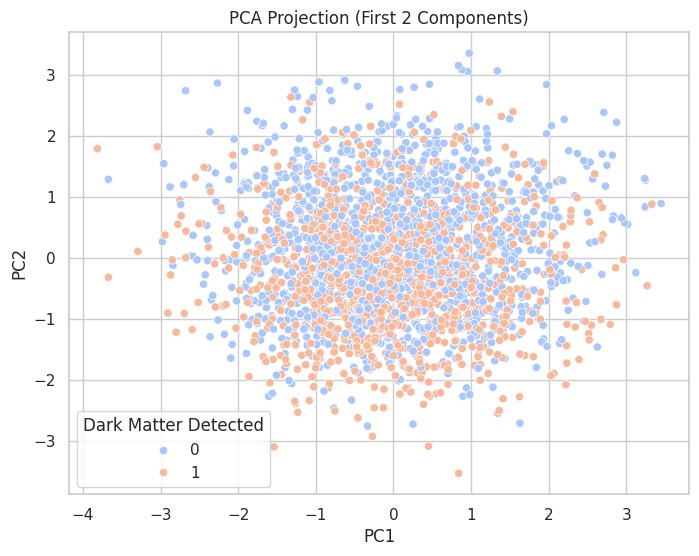
\includegraphics[width=1\linewidth]{Chap3/pca_projection.jpeg}
    \caption{First 2 component Projection}
    \label{fig:placeholder}
\end{figure}

This is a scatter plot that illustrates the data projected on to the first two principal components(PC1 and PC2) from PCA.

\begin{itemize}
    \item The x axis represents PC1 and the y axis denotes PC2.

    \item The data points are shaded whether or not dark matter is present, with blue representing "0" (no DM detection) and orange representing "1" (DM detection).

    \item This visualization allows checking how the first two components separate the two classes.
\end{itemize}
 
\section{Feature Selection and Engineering}

 

 \begin{figure}[H]
     \centering
     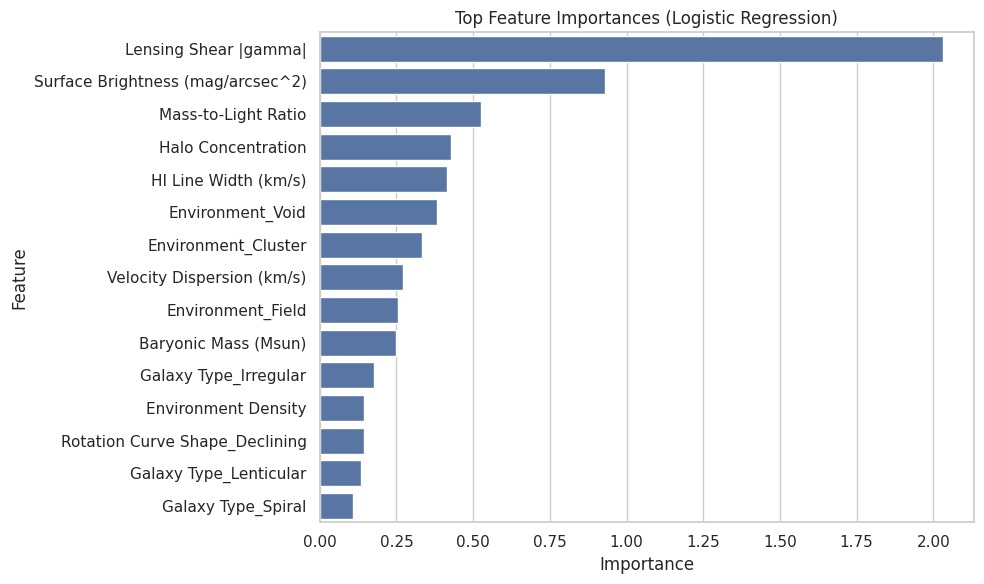
\includegraphics[width=1\linewidth]{image.png}
     \caption{Feature selection model}
     \label{fig:placeholder}
 \end{figure}
The chart you posted is the Top Feature Importances of a Logistic Regression model. It provides the importance of different features in predicting model output such as the length of bars suggest the corresponding significance.

\begin{itemize}
    \item The importance is highest for Lensing Shear [gamma]. This implies that gravitational lensing is the most important aspect of your model, meaning there is a strong correlation between lensing shear and the thing you are trying to predict (presumably dark matter or something like that)

    \item The Surface Brightness (mag/arcsec²) is next in priority. This means that the galaxies’ brightness per square arcsecond is an important factor in constraining the model’s prediction.

    \item Mass-to-Light Ratio and Halo Concentration are also big pieces of the puzzle, tells you that where the mass is as compared to light (how much dark matter there is relative to everything else) and how concentrated your galaxy’s halo matters.

    \item Other significant features are HI Line Width (km/s), Environment\_Void,Environment\_Cluster and Velocity Dispersion (km/s) that describe the environmental and dynamical properties of galaxies.

    \item Features such as Galaxy Type\_I rregular, Environment\_Density and Rotation Curve Shape\_Declining have some importance (ie contribute to the model) but they do it in a smaller way than the top features.

    \item Finally, Galaxy Type\_Lenticular and Galaxy Type\_Spiral have minor influence on the model performance,indicating that galaxy morphology may not be essential for this specific model.

\end{itemize}
 


\section{System Implementation}
\subsection{Performance Indicators}


Performance measures are critical to assess and compare the performance of machine learning model. They give the intuition about how well a model is doing on the problem you want it to solve. Performance measures comprise the accuracy, precision recall (sensitivity), F1 score, and model efficiency. And each of these metrics has a specific role to play in capturing some feature of the model behavior. These statistics are indispensable for both evaluating and refining the model to achieve optimal performance in a particular task.


\subsection{Analysis of the Confusion Matrix} 
The confusion matrix is a widely used technique to evaluate the classification models. It does gives a good in-depth breakdown of the true positives, true negates, false positives, and falls negatives. We can use the confusion matrix to compute a lot of performance metrics like accuracy, precision, recall and F1 score. The confusion matrix is a visual representation of how well the model is doing for classifying data to different classes, it makes it easy to identify where the model might be going wrong. This matrix is fundamental to interpret the strengths and weaknesses of the model on different category predictions.

 


\subsection{Accuracy}

Accuracy is the easiest and most straightforward performance measure. The ratio of correct predictions (True Positive + True Negative) to the total number of predictions made. On the other hand, accuracy provides a fast—but incomplete—picture of how a model is performing and can be misleading if the dataset is unbalanced. For example, in a very imbalanced dataset the model which always predicts the majority class can have high accuracy yet still suck at finding the minority class. Thus, accuracy should not be viewed in isolation but studied along with other metrics to have an integrated view of a model's performance.


\subsection{Precision}
Precision, just as a reminder that it’s sometimes called positive predictive value as well, is the rate at which our classifier generates true positives. It addresses the question: of all positive predictions by the model, how many were positive? Accuracy is crucial when false positives are cost-prohibitive or unjustifiable. If, say, a medical diagnosis model misclassifies healthy people as sick, it could prompt unnecessary tests or treatments. High precision indicates high trust in positive predictions.
\begin{table}[H]
\centering
\begin{tabular}{|l|c|c|}
\hline
\textbf{Model} & \textbf{Precision (0)} & \textbf{Precision (1)} \\
\hline
Decision Tree       & 0.76 & 0.71 \\\hline
Gradient Boosting   & 0.81 & 0.79 \\\hline
KNN                 & 0.73 & 0.72 \\\hline
Logistic Regression & 0.82 & 0.81 \\\hline
Naive Bayes         & 0.78 & 0.82 \\\hline
Random Forest       & 0.79 & 0.77 \\\hline
SVM                 & 0.79 & 0.77 \\\hline
XGBoost             & 0.79 & 0.76 \\
\hline
\end{tabular}
\caption{Precision for each model}
\end{table}





\subsection{Recall or Sensitivity}

Recall, or sensitivity, indicates the percentage of true positive instances that were accurately predicted by the model. e. true positives) the model was able to identify? Recall is particularly significant in the presence of severe costs associated with missing positive cases. For instance, in a fraud detection system not detecting fraudulent transactions (false negatives) might result in large losses. High recall means the model is catching as many of the true positive results as possible.
\begin{table}[H]
\centering
\begin{tabular}{|l|c|c|}
\hline
\textbf{Model} & \textbf{Recall (0)} & \textbf{Recall (1)} \\
\hline
Decision Tree       & 0.68 & 0.79 \\\hline
Gradient Boosting   & 0.78 & 0.82 \\\hline
KNN                 & 0.72 & 0.74 \\\hline
Logistic Regression & 0.80 & 0.82 \\\hline
Naive Bayes         & 0.83 & 0.77 \\\hline
Random Forest       & 0.76 & 0.80 \\\hline
SVM                 & 0.76 & 0.79 \\\hline
XGBoost             & 0.75 & 0.80 \\
\hline
\end{tabular}
\caption{Recall for each model}
\end{table}



\subsection{\textbf{F1 Score}}
The F1-score is the harmonic mean of precision and recall. It is a compromise between precision and recall that weights the two equally. F1 score is especially helpful when you have an uneven class distribution and moreover false positive and false negatives are of significant cost. Unlike accuracy which can be affected by a class imbalance, F1 score takes into account both the ability to identify positive cases (recall) and whether the predictions are correct or not (precision). A high F1 score means a model with good precision and recall.
 \begin{table}[H]
\centering
\begin{tabular}{|l|c|c|}
\hline
\textbf{Model} & \textbf{F1-Score (0)} & \textbf{F1-Score (1)} \\
\hline
Decision Tree       & 0.72 & 0.75 \\\hline
Gradient Boosting   & 0.79 & 0.80 \\\hline
KNN                 & 0.73 & 0.73 \\\hline
Logistic Regression & 0.81 & 0.82 \\\hline
Naive Bayes         & 0.80 & 0.79 \\\hline
Random Forest       & 0.77 & 0.79 \\\hline
SVM                 & 0.77 & 0.78 \\\hline
XGBoost             & 0.77 & 0.78 \\
\hline
\end{tabular}
\caption{F1-Score for each model}
\end{table}






